\chapter{Analysis}
\label{chap:analysis}

\xxx{From this point on, the document is a mess.}

\section{Analysis of Alternatives}\label{sec:alternatives}

In order to assess the potential benefits of the proposed virtual file system, it is essential to examine alternative solutions and compare their capabilities, limitations, and applicability.
This section will analyze existing non-virtual and virtual file systems with versioning and encryption features, as well as higher-level applications offering similar functionality.

Non-virtual versioning file systems is well documented concept, and there are several implementations available.
\xxx{At least describe some of the from \href{https://en.wikipedia.org/wiki/Versioning_file_system}{wikipedia page}}.

Furthermore, several virtual file systems (VFS) with versioning capabilities have been developed:

\begin{itemize}
    \item User space file systems implemented with FUSE:
    \begin{itemize}
        \item \href{https://github.com/FooSoft/vfs}{A simple versioning file system for Linux using FUSE}, written in Go.
        \item \href{https://www.usenix.org/legacy/events/usenix04/tech/freenix/cornell.html}{Wayback: A User-level Versioning File System for Linux}, developed in Perl for the USENIX 2004 Annual Technical Conference using an older version of FUSE.
    \end{itemize}
    \item \href{https://osm.hpi.de/vvfs/}{Copy-on-Write Version Support for VFS under Linux} by Stephan Müller and Sven Widmer, implemented as a kernel patch.
    \item \href{https://wiki.tcl-lang.org/page/A+versioning+virtual+filesystem}{A versioning virtual filesystem by Steve Huntley}, written in Tcl.
    However, this solution primarily serves as a language demonstration rather than a practical implementation.
\end{itemize}

These existing solutions have various constraints, such as being platform-specific (mainly Linux-only) or discontinued.
While VFS with encryption is less common, there also exists a non-virtual alternative as \ldots % https://learn.microsoft.com/en-gb/windows/win32/fileio/file-encryption?redirectedfrom=MSDN
The closest example to the desired functionality is \href{https://github.com/rmind/rvault}{rvault}, which focuses on encrypting small files (passwords, keys, and secrets) and makes them accessible through one-time password authentication.
However, this does does differ from the intended functionality of the proposed VFS.

The main competition thus stems from higher-level applications that provide versioning and encryption features.
These applications have their own set of limitations, such as requiring a constantly running background program with access to all files and offering limited extensibility for incorporating other features.
In most instances, integrating additional functionalities into these applications would not be practical or feasible.

Despite the limitations of existing solutions, it is worth noting that some operating systems, specifically macOS, provide built-in support for versioning and encryption features.
MacOS's Time Machine offers versioning capabilities, allowing users to revert to previous versions of files or restore deleted data.
Furthermore, macOS incorporates FileVault, a native full-disk encryption solution that secures data.
However, these features are not available on other platforms, and they may not provide the desired level of control over the process.

\section{FUSE: Rationale and Alternatives}\label{sec:fuse-analysis}

In the development of a virtual file system, there are two primary approaches to consider: writing kernel drivers or utilizing a user space library.
Writing kernel drivers provides low-level access to the operating system, but it requires extensive knowledge of the kernel, as well as platform-specific implementations.
This method can be time-consuming, error-prone, and challenging to maintain.

An alternative to writing kernel drivers is a library such as using FUSE, a popular tool for creating virtual file systems in user space without modifying kernel code.
FUSE offers a comprehensive API for defining file system operations, making it an appropriate choice for building a VFS.
It allows developers to focus on the functionality and logic of their custom file system, rather than the intricate details of kernel programming.
Yet, FUSE is not without its limitations.
It is arguable whether it is the best choice for a C++ implementation, as it is written in C, but more on that later.

Although FUSE was initially designed for Linux, variants are available for other platforms, ensuring cross-platform compatibility:

\begin{itemize}
    \item \textbf{Linux}: \href{https://github.com/libfuse/libfuse}{libfuse} - The reference implementation of FUSE.
    \item \textbf{macOS}: \href{https://osxfuse.github.io/}{FUSE for macOS} - A macOS port of FUSE.
    \item \textbf{Windows}: \href{https://github.com/billziss-gh/winfsp}{WinFsp} - A Windows File System Proxy that provides FUSE-compatible functionality.
\end{itemize}

To develop a new file system using FUSE, a handler program connected to the provided libfuse library must be created.
The primary objective of this handler program is to define the file system's behavior in response to read, write, and stat requests.
Additionally, the handler program is responsible for mounting the new file system.
Upon mounting, the handler is registered with the kernel.
When a user initiates read, write, or stat requests for the newly mounted file system, the kernel forwards these I/O requests to the handler, which processes them accordingly.
The handler's response is then relayed back to the user by the kernel, ensuring a seamless interaction between the custom file system and the operating system.

\begin{figure}[ht]
    \centering
    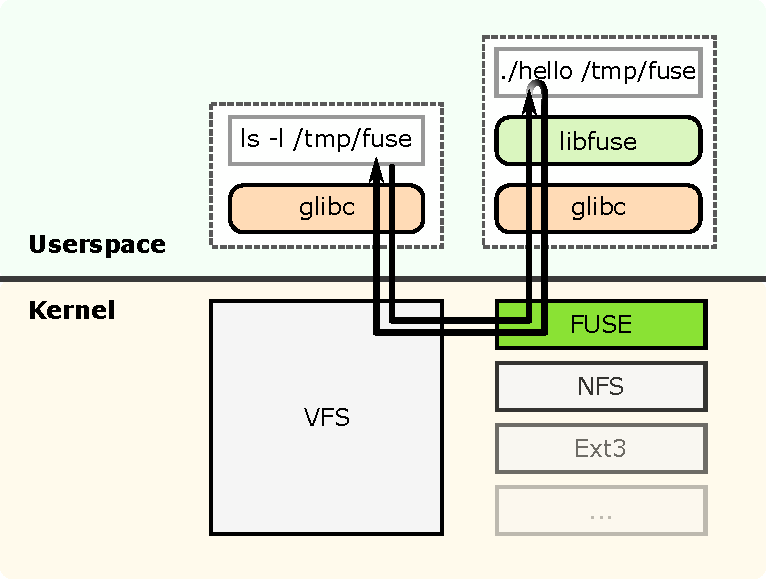
\includegraphics[width=\linewidth]{img/fuse_diagram}
    \caption{FUSE flow-chart diagram}
    \label{fig:fuse-diagram}
\end{figure}

Considering the advantages of user space development and the availability of FUSE for multiple platforms, FUSE is the preferred choice for implementing the proposed VFS.
This approach enables the development of a cross-platform VFS with versioning and encryption capabilities while avoiding the complexity of kernel driver development.

\section{Other libraries}\label{sec:other-libraries-analysis}

While FUSE serves as the foundation for the VFS implementation, several other libraries will be employed to address various aspects of the project.

\subsection{Encryption}\label{subsec:encryption-analysis}

\href{https://www.cryptopp.com/}{Crypto++} is a comprehensive, open-source C++ class library that provides a wide array of cryptographic schemes, including encryption, hashing, and authentication algorithms.\ By incorporating Crypto++ into the project, file-level encryption can be implemented within the VFS, ensuring the security and privacy of stored data.

\subsection{Testing}\label{subsec:gtest}

\href{https://github.com/google/googletest}{Google Test}, also known as gtest, is a popular and versatile C++ testing framework developed by Google.\ This library allows for efficient testing of individual components and the overall functionality of the VFS. Through the use of gtest, the quality, reliability, and performance of the custom VFS can be assessed, ensuring that it meets the requirements and expectations outlined in this thesis.
\ldots

\section{Build system and multiplatform challenges}\label{sec:build-system-and-multiplatform-challenges}

Use of CMake, problem with M1 Mac and Windows\ldots even though portable